
\documentclass[12pt]{article}

\usepackage[spanish]{babel}
\usepackage{hyperref}
\usepackage{graphicx}
\usepackage{listings}
\usepackage{color}
\usepackage{multicol}
\usepackage{amssymb}
\usepackage{enumitem}
\usepackage{here}
\usepackage{dsfont}
\usepackage{amsmath}
\usepackage{tipa}
\usepackage{float}
\usepackage{tikz}
\spanishdecimal{.}

\title{Matemáticas para las Ciencias Aplicadas I}
\title{
	Tercera Lista de Problemas \\
	\textbf{Primera  Parte} \\
	\vspace{1ex}
	\large Matemáticas para las Ciencias Aplicadas I \\
	Facultad de Ciencias, UNAM}

\date{\today}

\author{Flores Morán Julieta Melina \\ Zarco Romero José Antonio}

\begin{document}

\maketitle

%% De la sección 3.2: ejercicios 38 y 57.
%% De la sección 3.3: ejercicios 54, 70, 76 y 83.
%% De la sección 3.4: ejercicios 23, 36, 45 y 47.
 %% De la sección 3.6: ejercicios 58, 63 y 65

%% 3.2 -------------------------------------------------------------------------------------------------------------------------------------------------------------------------------------------------------------------------------
\section{Sección 3.2 \\ Derivadas De Funciones Logarítmicas}
% 38 -------------------------------------------------------------------------------------------------------------
\subsection{Ejercicio 38} Flores Morán Julieta Melina \\

Encuentre $dy/dx$ usando diferenciación logarítmica.
\[
y=\frac{\sin{x}\cos{x}\tan^3{x}}{\sqrt{x}}
\]
\begin{equation*}
  \begin{split}
  \ln(y)
  &= \ln(\sin{x}\cos{x}\tan^3{x})-\ln(\sqrt{x}) \\
  &= \ln(\sin{x})+\ln(\cos{x})+\ln(\tan^3{x})-\ln \left(x^{\frac{1}{2}}\right) \\
  &= \ln(\sin{x})+\ln(\cos{x})+3\ln(\tan{x})-\frac{1}{2}\ln x \\
  \frac{1}{y}\frac{dy}{dy}
  &= \frac{\cos{x}}{\sin{x}} + \frac{-\sin{x}}{\cos{x}} + \frac{3\sec^2{x}}{\tan{x}} - \frac{1}{2x} \\
  \frac{dy}{dy}
  &= y \left[ \cot{x}-\tan{x} + \frac{3\sec^2{x}}{\tan{x}} - \frac{1}{2x} \right] \\
  \therefore \frac{dy}{dy}
  &= \frac{\sin{x}\cos{x}\tan^3{x}}{\sqrt{x}}
  \left[ \cot{x}-\tan{x} + \frac{3\sec^2{x}}{\tan{x}} - \frac{1}{2x} \right] \\
  \end{split}
\end{equation*}

% 57 -------------------------------------------------------------------------------------------------------------
\subsection{Ejercicio 57} Zarco Romero José Antonio \\

Sea $p$ el número de paramecios en una solución nutritiva $t$ días después del inicio de un experimento, y supongamos que $p$ es definido implícitamente como una función de $t$ por la ecuación
\[
0 = \ln p + 0.83 − \ln(2.3-
0.0046p) − 2.3t
\]
Utilice la diferenciación implícita para demostrar que la tasa de cambio de $p$ con respecto a $t$ satisface la ecuación
\[
\frac{dp}{dt} = 0.0046p(500-p)
\]
\begin{equation*}
  \begin{split}
    \ln p - \ln(2.3 − 0.0046p)
    &= 2.3t -0.83 \\
    \frac{1}{p}\frac{dp}{dt}+\frac{0.0046}{2.3-0.0046p}\frac{dp}{dt}
    &= 2.3 \\
    \frac{dp}{dt}\left[\frac{1}{p}+\frac{0.0046}{2.3-0.0046p}\right]
    &= 2.3 \\
    \frac{dp}{dt}\left[\frac{2.3-0.0046p+ 0.0046p}{p(2.3-0.0046p)}\right]
    &= 2.3 \\
    \frac{dp}{dt}\left[\frac{2.3}{2.3p-0.0046p^2}\right]
    &= 2.3 \\
    \frac{dp}{dt}
    &= 2.3\left[\frac{2.3p-0.0046p^2}{2.3}\right] \\
    &= 2.3p-0.0046p^2 \\
    \therefore \frac{dp}{dt}
    &= 0.0046p(500-p)
  \end{split}
\end{equation*}

%% 3.3 -----------------------------------------------------------------------------------------------------------------------------------------------------------------------------------------------------------------------------
\section{Sección 3.3 \\ Derivadas De Funciones Trigonométricas Exponenciales E Inversas} 
% 54 -------------------------------------------------------------------------------------------------------------
\subsection{Ejercicio 54} Zarco Romero José Antonio \\

Encuentre $\frac{dy}{dx}$.
\[
y=x^2(\sin^{-1}{x})^3
\]
\begin{equation*}
  \begin{split}
    \frac{dy}{dx}
    &= \left[x^2\cdot \frac{d}{dx}(\sin^{-1}{x})^3 \right] + \left[(\sin^{-1}{x})^3\cdot \frac{d}{dx}x^2\right] \\
    &= \left\lbrace x^2\cdot \left[3(\sin^{-1}{x})^2\cdot \frac{d}{dx}(\sin^{-1}{x}) \right] \right\rbrace + \left[(\sin^{-1}{x})^3\cdot 2x\right] \\
    &= \left\lbrace x^2\cdot \left[3(\sin^{-1}{x})^2\cdot \frac{1}{\sqrt{1-x^2}} \right] \right\rbrace + \left[2x(\sin^{-1}{x})^3\right] \\
    &= \left\lbrace x^2\cdot \left[ \frac{3(\sin^{-1}{x})^2}{\sqrt{1-x^2}} \right] \right\rbrace + 2x(\sin^{-1}{x})^3 \\
    \therefore
    \frac{dy}{dx}
    &= \frac{3x^2(\sin^{-1}{x})^2}{\sqrt{1-x^2}} + 2x(\sin^{-1}{x})^3 \\
  \end{split}
\end{equation*}

% 70 -------------------------------------------------------------------------------------------------------------
\subsection{Ejercicio 70} Flores Morán Julieta Melina \\

Sea $f(x)=\frac{exp(4-x^2)}{x}$, $x>0$.
\begin{enumerate}
\item Demuestre que $f$ es uno a uno. \\
Para demostrar que la función f es uno a uno basta con demostrar que es creciente o decreciente en todo el dominio su f, lo que se deduce si la derivada no cambia de signo en ningún valor del dominio.

\begin{equation*}
  \begin{split}
    f'(x)
    &=  \frac{d}{dx} \left[\frac{1}{x} \cdot e^{4-x^2}\right] \\
    &= \left[\frac {1}{x}\cdot \frac{d}{dx}(e^{4-x^2}) \right] + \left[e^{4-x^2}\cdot \frac{d}{dx}(x^{-1})\right] \\
    &= \left\lbrace \frac{1}{x} \cdot \left[e^{4-x^2} \cdot \frac{d}{dx}(4-x^2) \right] \right\rbrace + \left[e^{4-x^2}(-x^{-2})] \\
    &=  \left\lbrace \frac{1}{x} \cdot \left[e^{4-x^2} ( -2x) \right] \right\rbrace + \left[e^{4-x^2}(-x^{-2})] \\
    &= \frac{-2x \cdot e^{4-x^2}}{x} - \frac {e^{4-x^2}}{x^{2}}= \frac{x(-2x  e^{4-x^2})- e^{4-x^2} }{x^2}\\
    &= \frac{-e^{4-x^2} (2x^{2}+1) }{x^2} = -e^{4-x^2} ( \frac{2x^{2}+1}{x^2} )\\
     &=  -e^{4-x^2}( \frac{2x^{2}}{x^2} +\frac{1}{x^2}) =   -e^{4-x^2} (2 +\frac{1}{x^2})\\
    \therefore
    f'(x) 
    & =  -e^{4-x^2} (2 +\frac{1}{x^2})  \\
  \end{split}
\end{equation*}

Los factores $ e^{4-x^2}$  y  $2 +\frac{1}{x^2}$ siempre serán positivos para toda x. Por lo que al multiplicarlo por -1 podemos aseverar que: \\
  $f'(x) <0 $ para toda x.\\
  Sabiendo que la derivada no cambia de signo en todo el dominio de la función, y que la función es decreciente en todo el dominio queda demostrado que f es una función uno a uno.\\
  
\item Sea $g(x)=f^{-1}(x)$ y defina $F(X)=f([g(x)]^2)$. Encuentre $F'\left(\frac{1}{2}\right)$
  
 \begin{equation*}
  \begin{split}
    F'(x)
    &= \frac{d}{dx} \left[ f([g(x)]^2) \right] \\
    &= f'([g(x)]^2) \cdot  \frac{d}{dx} \left[g(x)^2\right] \cdot g'(x) \\
    &= f'([g(x)]^2) \cdot  2g(x) \cdot g'(x) \\
    &= f'([f^{-1}(x)]^2) \cdot  2f^{-1}(x) \cdot (f^{-1})'(x) \\
    \text{Podemos hacer uso de la fórmula } \\
    (f^{-1})'(x) = \frac{1}{f'(f^{-1}(x))}\\
    &= f'([f^{-1}(x)]^2) \cdot  2f^{-1}(x) \cdot \frac{1}{f'(f^{-1}(x))} \\
  \end{split}
\end{equation*}

Notemos que para poder resolver  $F'\left(\frac{1}{2}\right)$ necesitaremos conocer el valor de $f^{-1}\left(\frac{1}{2}\right)$. Consideremos entonces que:\\
  \[
  f(2) = \frac{e^{4-2^2}}{2} = \frac{e^{4-4}}{2} = \frac{e^{0}}{2} = \frac{1}{2}
  \]
  Por lo tanto, ya que $f(2) = \frac{1}{2}$, entonces  $f^{-1}\left(\frac{1}{2}\right) = 2$.\\
  Con esta información, procedemos a evaluar en $\frac{1}{2}$.


\begin{equation*}
  \begin{split}
    F'\left(\frac{1}{2}\right)
    &=  f'([f^{-1}(x)]^2) \cdot  2f^{-1}(x) \cdot \frac{1}{f'(f^{-1}(x))} \vline _{x=\frac{1}{2}} \\
    &=   f'([f^{-1} \left(\frac{1}{2}\right)]^2) \cdot  2f^{-1}\left(\frac{1}{2}\right) \cdot \frac{1}{f'(f^{-1}\left(\frac{1}{2}\right))}  \\
    &=   f'([2]^2) \cdot  2\cdot 2 \cdot \frac{1}{f'(2)}  \\
    &=   f'(4) \cdot 4 \cdot \frac{1}{f'(2)}  
    =  4 \cdot \frac{ f'(4)}{f'(2)}  \\
    &=  4 \cdot \frac{  -e^{4-4^2} (2 +\frac{1}{4^2}) }{ -e^{4-2^2} (2 +\frac{1}{2^2})}  
    =  4 \cdot \frac{e^{4-16} (2 +\frac{1}{16}) }{e^{4-4} (2 +\frac{1}{4})}  \\
    &=  4 \cdot \frac{e^{-12} (\frac{33}{16}) }{e^{0} (\frac{9}{4})}  
    =  4 \cdot e^{-12} \frac{\frac{33}{16}}{ 1\cdot (\frac{9}{4})}  \\
    &=  4 \cdot \frac{1}{e^{12}} \cdot \frac{\frac{33}{16}}{ \frac{9}{4}}  
    =  \frac{4}{e^{12}} \cdot \frac{4 \cdot 33}{9\cdot 16} 
    =  \frac{ 4 \cdot 4 \cdot 33}{9\cdot 16\cdot e^{12}} \\
    &=  \frac{11}{3e^{12}} \\
    \therefore
   F'\left(\frac{1}{2}\right)
    & = \frac{11}{3e^{12}}  \\
  \end{split}
\end{equation*}

\end{enumerate}

% 76 -------------------------------------------------------------------------------------------------------------
\subsection{Ejercicio 76} Flores Morán Julieta Melina \\

Supongamos que la población de bacterias dependientes de oxígeno en un estanque se modela mediante la ecuación
\[
P(t)=\frac{60}{5+7e^{-t}}
\]
donde $P(t)$ es la población (en miles de millones) $t$ días después de una observación inicial en el momento $t = 0$.
\begin{enumerate}
\item Utilice una herramienta gráfica para representar gráficamente la función $P(t)$.
  \begin{figure}[H]
\centering
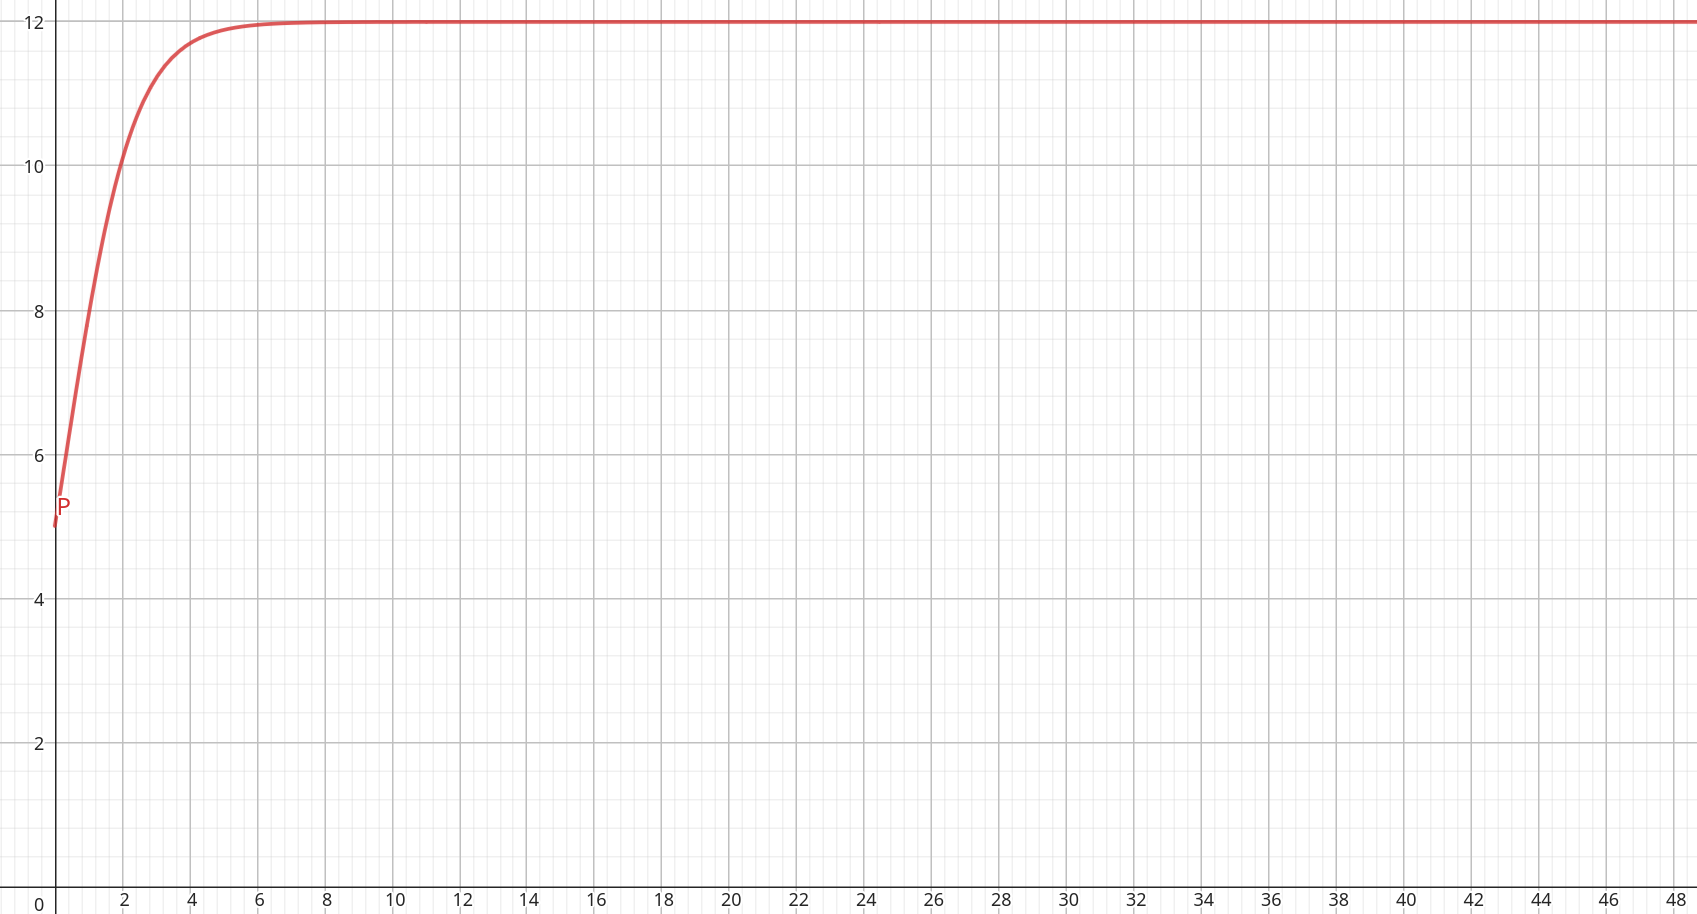
\includegraphics[width=0.6\textwidth]{../img/img_Lista3/poblacionT.png}
  \end{figure}
 Figura: Gráfica de la función P(t).
\item Explique con palabras qué le sucede a la población a lo largo del tiempo. Comprueba tu conclusión encontrando $\lim_{t \to +\infty} P(t)$.\\
  En la gráfica se puede observar que la población se acerca a 12 miles de millones a medida que pasan los días pero nunca pasa de esta cantidad.Esto quiere decir que la población tiende a 12 conforme t crece.\\


\[ \begin{equation*}
  \begin{split}
    \lim_{t \to +\infty} P(t)
    &= \lim_{t \to +\infty} \frac{60}{5+7e^{-t}} \\
    &= \frac{ \lim_{t \to +\infty} 60}{ \lim_{t \to +\infty} (5+7e^{-t})} \\
    &= \frac{ 60}{ \lim_{t \to +\infty}5+  \lim_{t \to +\infty} 7e^{-t}} \\
   & =  \frac{ 60}{ 5+ 7  \lim_{t \to +\infty} e^{-t}}
 \end{split}
\end{equation*} \]
  
    Ya que $ \lim_{t \to +\infty} e^{-t} = 0$
    \[
    \begin{equation*}
  \begin{split}
     \frac{ 60}{ 5+ 7 \cdot 0} =  \frac{60}{5} = 12
        \end{split}
\end{equation*}
\]
Este resultado comprueba que por más grande que el valor de t se vuelva, la población tiende a 12 miles de millones.\\

\item3.  En palabras, ¿qué sucede con la \textit{tasa} de crecimiento de la población a lo largo del tiempo? Comprueba tu conclusión graficando $P'(t)$.\\
  La tasa es creciente por un tiempo y después disminuye tendiendo a volverse 0 ya que la población tiende a no crecer y quedarse en 12 miles de millones, la tasa de crecimiento tiende a ser 0.\\
 
       Para comprender el comportamiento de  la tasa de crecimiento, que sería $P'(t)$, conviene  calcularla.
\[ \begin{equation*}
  \begin{split}
    P'(t) = \frac{d}{dt} \left[ 60 \cdot (5+7e^{-t})^{-1}\right]\\
    &= 60 \cdot \frac{d}{dt}\left[(5+7e^{-t})^{-1}\right]\\
    &=  60 \cdot -(5+7e^{-t})^{-2} \cdot \frac{d}{dt} (5+7e^{-t}) \\
    &= 60 \cdot -(5+7e^{-t})^{-2} \cdot 7 \cdot  \frac{d}{dt}e^{-t}\\
    &= 60 \cdot -(5+7e^{-t})^{-2} \cdot 7 \cdot  -e^{-t} \\
    &= 60 \cdot \frac {1}{(5+7e^{-t})^{2}} \cdot 7 \cdot  e^{-t}\\
    &=  \frac {420 \cdot  e^{-t}}  {(5+7e^{-t})^{2}} =  \frac {\frac{420}{e^{t}}}  {(5+\frac{7}{e^{t}})^{2}}\\
    &=  \frac {420}  {(\frac{5e^{t}+7}{e^{t}})^{2} \cdot e^{t}} = \frac {420}  {\frac{(5e^{t}+7)^{2}}{e^{2t}} \cdot e^{t}} =
    \frac {420}{\frac{(5e^{t}+7)^{2}}{e^{t}}} =  \frac {420\cdot e^{t}}{(5e^{t}+7)^{2}}
     \end{split}
\end{equation*} \]

Con esta información, podemos auxiliarnos del  $\lim_{t \to +\infty} P'(t)$ para conocer cómo es la tasa de crecimiento mientras avanza el tiempo.\\
\[ \begin{equation*}
  \begin{split}
    \lim_{t \to +\infty} P'(t) = \lim_{t \to +\infty}   \frac {420\cdot e^{t}}{(5e^{t}+7)^{2}}  = \frac{ \lim_{t \to +\infty} 420\cdot e^{t} }{ \lim_{t \to +\infty} (5e^{t}+7)^{2}} = \frac{\infty}{\infty}
 \end{split}
\end{equation*} \]
Ya que da lugar a esta indeterminación podemos usar la regla de L'Hôpital.\\
\[ \begin{equation*}
  \begin{split}
    \frac {  \frac{d}{dt}  (420\cdot e^{t})}{  \frac{d}{dt}  \left[(5e^{t}+7)^{2}\right]}  = \frac {420\cdot e^{t}}{ 2(5e^{t}+7) \cdot 5e^{t}} =
   \frac {420\cdot e^{t}}{50e^{2t}+70e^{t}} =  \frac {42}{5e^{t}+7}
 \end{split}
\end{equation*} \]

\[ \begin{equation*}
  \begin{split}
    \lim_{t \to +\infty} P'(t) = \lim_{t \to +\infty}  \frac {42}{5e^{t}+7}  = \frac{ \lim_{t \to +\infty} 42}{ \lim_{t \to +\infty} 5e^{t}+7 } = \frac{42}{\infty} = 0
 \end{split}
\end{equation*} \]
Con esto demostramos que la tasa de crecimiento tiende a volverse 0 a lo largo del tiempo, comportamiento que se observa en la gráfica siguiente.
   \begin{figure}[H]
\centering
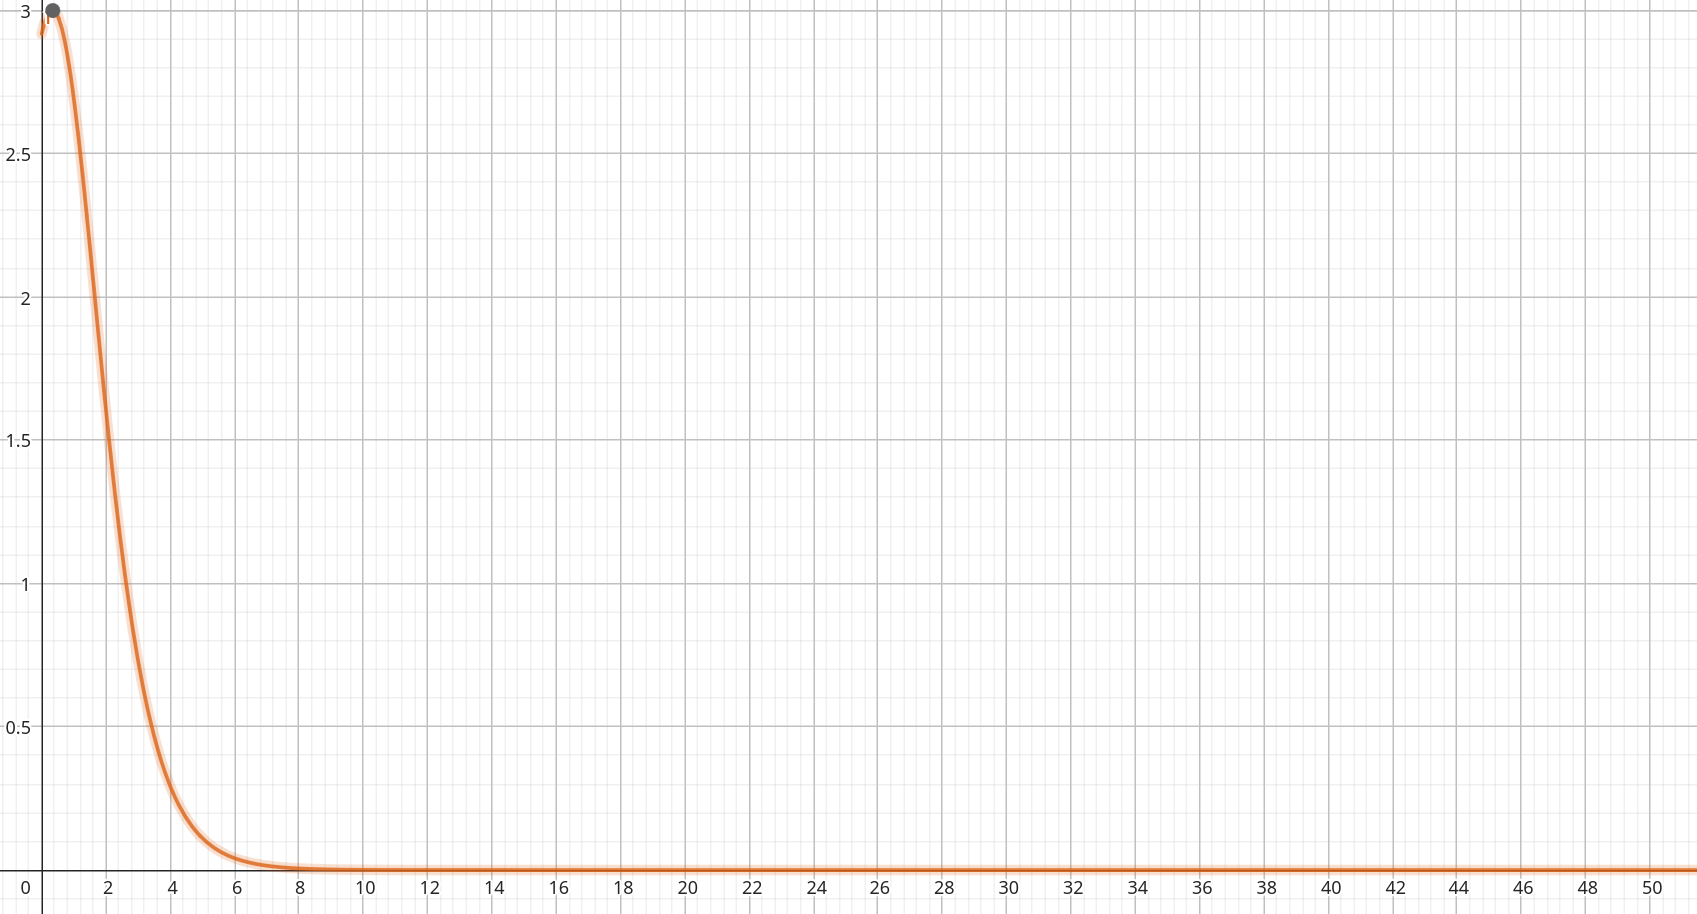
\includegraphics[width=0.6\textwidth]{../img/img_Lista3/tasa.png}
     \end{figure}
     Figura: Gráfica de $P'(t)$.
\end{enumerate}

% 83 -------------------------------------------------------------------------------------------------------------
\subsection{Ejercicio 83} Zarco Romero José Antonio \\

Supongamos que un rodamiento  de bolas de acero se suelta dentro de una tina de fluido y comienza a hundirse. Según un modelo, la velocidad $v(t)$ (en $m/s$) del rodamiento de bolas $t$ segundos después de su liberación viene dada por la fórmula
\[
v(t)=\frac{9.8}{k}(1-e^{-kt})
\]
donde $k$ es una constante positiva que corresponde a la resistencia que ofrece el fluido contra el movimiento del rodamiento. (Cuanto menor sea el valor de $k$, más débil será la resistencia).
Para $t$ fijo, determine el valor límite de la velocidad cuando $k\rightarrow 0^+$ y dé una interpretación física del límite.
\[ \begin{equation*}
  \begin{split}
    \lim_{k \to 0^+} v(t)
    &= \lim_{k \to 0^+} \left[ \frac{9.8}{k}(1-e^{-kt}) \right] \\
    &= 9.8 \lim_{k \to 0^+} \frac{1-e^{-kt}}{k} \\
    & \qquad \text{Aplicando la serie de MacLaurin, tenemos que:} \\
    &= 9.8 \lim_{k \to 0^+} \frac{1-
      \left(1+\frac{(-kt)}{1!}+\frac{(-kt)^2}{2!}+\frac{(-kt)^3}{3!}+\ldots \right)
    }{k} \\
    &= 9.8 \lim_{k \to 0^+} \frac{1-
      \left(1-kt+\frac{(kt)^2}{2!}-\frac{(kt)^3}{3!}+\ldots \right)
    }{k} \\
    &= 9.8 \lim_{k \to 0^+} \frac{kt-\frac{(kt)^2}{2!}+\frac{(kt)^3}{3!}-\ldots}{k} \\
    &= 9.8 \lim_{k \to 0^+} \left[ t-\frac{k(t)^2}{2!}+\frac{k^2t^3}{3!}-\ldots \right] \\
    &= 9.8 ( t-0+0-\ldots ) \\
    \therefore
    \lim_{k \to 0^+} v(t)
    &= 9.8 t \\
  \end{split}
\end{equation*} \]

Esto significa que si el fluido no ofrece resistencia, entonces la velocidad aumentará a una tasa constante de $9.8 m/s$.

%% 3.4 -----------------------------------------------------------------------------------------------------------------------------------------------------------------------------------------------------------------------------
\section{Sección 3.4 \\ Tasas Relacionadas} 
% 23 -------------------------------------------------------------------------------------------------------------
\subsection{Ejercicio 23} Flores Morán Julieta Melina \\

\begin{figure}[H]
\centering
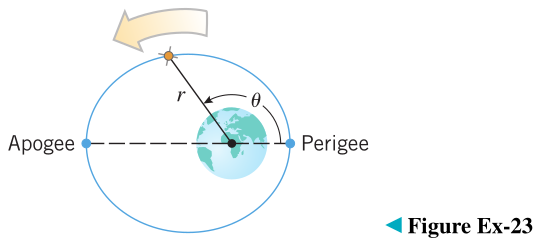
\includegraphics[width=0.6\textwidth]{../img/img_Lista3/23.png}
\end{figure}
Un satélite se encuentra en una órbita elíptica alrededor de la Tierra. Su distancia $r$ (en millas) desde el centro de la Tierra está dada por
\[
r=\frac{4995}{1+0.12\cos{\theta}}
\]
donde $\theta$ es el ángulo medido desde el punto de la órbita más cercano a la superficie de la Tierra (consulte la figura adjunta).
\begin{enumerate}
\item Encuentre la altitud del satélite en el \textit{\textbf{perigeo}} (el punto más cercano a la superficie de la Tierra) y en el \textit{\textbf{apogeo}} (el punto más alejado de la superficie de la Tierra). Utilice $3960~  mi$ como radio de la Tierra.\\
La altitud del satélite será la distancia desde la corteza de la tierra hasta el sátelite. Es decir, r menos el radio de la tierra dado como $3960~  mi$.\\ En el perigeo el ángulo $\theta$ vale 0 rad. Por lo tanto la distancia desde el centro de la Tierra será:
 
\begin{equation*}
  \begin{split}
    r
    &= \frac{4995}{1+0.12\cos{0}}\\
    &= \frac{4995}{1+0.12\cdot 1}\\
    &= \frac{4995}{1.12}\\
    &= 4459.8214\\
    \therefore
    r
    &= 4459.8214 ~ mi  \\
  \end{split}
\end{equation*}

Con este dato, ya podemos calcular la altitud en el perigeo.

\begin{equation*}
  \begin{split}
    \text{altitud en el perigeo}
    &= r - 3960 \\
    &= 4459.8214 - 3960\\
    \therefore
    altitud
    &= 499.8214 ~ mi  \\
  \end{split}
\end{equation*}

Gracias a la figura, es fácil notar que $\theta$ durante el apogeo vale $180^{\circ}$ o  $\pi$ rad. Siguiendo un procedemiento análogo al anterior, podemos calcular la altitut restando 3960 mi de lo que obtengamos para r dado este ángulo.
\begin{equation*}
  \begin{split}
    r
    &= \frac{4995}{1+0.12\cos{\pi}}\\
    &= \frac{4995}{1+0.12\cdot -1}\\
    &= \frac{4995}{1 - 0.12}\\
    &= \frac{4995}{0.88}\\
    \therefore
    r
    &= 5676.1363 ~ mi \\
  \end{split}
\end{equation*}

Con este dato, ya podemos calcular la altitud en el apogeo.

\begin{equation*}
  \begin{split}
    \text{altitud en el apogeo}
    &= r - 3960 \\
    &=  5676.1363 - 3960\\
    \therefore
    altitud
    &= 1716.136364 ~ mi \\
  \end{split}
\end{equation*}

\item En el instante en que $\theta$ es $120^{\circ}$, el ángulo $\theta$ aumenta a razón de $2.7^{\circ} /min$. Encuentre la altitud del satélite y la velocidad a la que cambia la altitud en este instante. Exprese la velocidad en unidades de $mi/min$.\\
Primero convine tener los ángulos dados radianes.
  \[
  120^{\circ} =  120^{\circ} \left( \frac{\pi rad}{180 ^{\circ}} \right) = \frac{2\pi}{3} rad
  \]
   \[
  2.7^{\circ} =  2.7^{\circ} \left( \frac{\pi rad}{180 ^{\circ}} \right) = \frac{3\pi}{200} rad
   \]

   \\La altitud del satélite en el ángulo dado se calcula restando la distancia desde el centro de la Tierra menos el radio de la misma.

   \begin{equation*}
  \begin{split}
    r
    &= \frac{4995}{1+0.12\cos{\frac{2\pi}{3}}}\\
    &= \frac{4995}{1+0.12\cdot - \frac{1}{2}}\\
    &= \frac{4995}{1 - 0.06}\\
    &= \frac{4995}{0.94}\\
    \therefore
    r
    &= 5313.829787 ~ mi \\
  \end{split}
\end{equation*}

Con este dato, ya podemos calcular la altitud en el apogeo.

\begin{equation*}
  \begin{split}
    \text{altitud en el apogeo}
    &= r - 3960 \\
    &=  5676.1363 - 3960\\
    \therefore
    altitud
    &= 1716.136364 ~ mi \\
  \end{split}
\end{equation*}

\\ Para encontrar la tasa de cambio de la altitud con respecto al tiempo. Podemos derivar implicitamente la fórmula de la altitud que podemos describir como :
\[
a = \frac{4995}{1+0.12\cos{\theta}} - 3960
\]

\begin{equation*}
  \begin{split}
  \frac{da}{dt}
    &= \frac{d}{dt}\left[\frac{4995}{1+0.12\cos{\theta}}-3960\right]\\
  &= \frac{d}{dt}\left[4995 \cdot (1+0.12\cos{\theta})^{-1}\right]- \frac{d}{dt} (3960)\\
  &= \frac{d}{dt}\left[4995 \cdot (1+0.12\cos{\theta})^{-1}\right]\\
  &= 4995 \cdot \frac{d}{dt}\left[(1+0.12\cos{\theta})^{-1}\right]\\
  &= 4995 \cdot \left[-(1+0.12\cos{\theta})^{-2} \cdot -0.12sen\theta \cdot   \frac{d\theta}{dt}  \right]\\
   &=  4995 \cdot (1+0.12\cos{\theta})^{-2} \cdot 0.12sen\theta \cdot   \frac{d\theta}{dt}  \\
    \therefore
   \frac{da}{dt} 
   &= \frac{dr}{dt} 
   = \frac{4995 \cdot  0.12sen\theta }{(1+0.12\cos{\theta})^{2}}  \cdot   \frac{d\theta}{dt} \\
  \end{split}
\end{equation*}

Evaluada en ese instante dónde sabemos que  $\theta =  \frac{2\pi}{3} ~ rad $ y $\frac{d\theta}{dt} = \frac{3\pi}{200} ~ rad/min $ tenemos que:

\begin{equation*}
  \begin{split}
  \frac{da}{dt} \vline _{\theta = \frac{2\pi}{3} }
  &=\frac{4995 \cdot  0.12sen\theta }{(1+0.12\cos{\theta})^{2}}  \cdot   \frac{d\theta}{dt}  \vline _{\theta = \frac{2\pi}{3} } \\
  &=\frac{4995 \cdot  0.12sen\theta }{(1+0.12\cos{\theta})^{2}}  \cdot    \frac{3\pi}{200}  \vline _{\theta = \frac{2\pi}{3} } \\
  &=\frac{4995 \cdot  0.12\sin{\frac{2\pi}{3}} }{(1+0.12\cos{\frac{2\pi}{3}})^{2}}  \cdot    \frac{3\pi}{200}  \\
  &=587.478075  \cdot    \frac{3\pi}{200}  \\
  &=27.68425207  \\
  \therefore
   \frac{da}{dt} \vline _{\theta = \frac{2\pi}{3} }
     &=27.68425207 ~ mi/min \\
  \end{split}
\end{equation*}


\end{enumerate}

% 36 -------------------------------------------------------------------------------------------------------------
\subsection{Ejercicio 36} Zarco Romero José Antonio \\

Un helicóptero de la policía vuela hacia el norte a $100 mi/h$ y a una altitud constante de $\frac{1}{2} mi$. A continuación, un automóvil viaja hacia el oeste por una carretera a $75 mi/h$. En el momento en que el helicóptero cruza la carretera, el automóvil se encuentra a 2 millas al este del helicóptero.
\begin{enumerate}
\item ¿A qué velocidad cambia la distancia entre el automóvil y el helicóptero en el momento en que el helicóptero cruza la carretera?

Se nos da la velocidad constante con la que viajan un helicóptero y un automóvil por una carretera. Así, sea
\begin{itemize}
\item $t=$ Número de horas transcurridas desde los comienzos de los respectivos vehículos.
\item $z=$ La distancia entre el automóvil y el helicóptero.
\item $x=$ La distancia horizontal entre el automóvil y el helicóptero.
\item $y=$ La distancia entre el helicóptero y la carretera.
\item $d=\frac{1}{2} mi$ La altitud del helicóptero.
\end{itemize}
Sabemos las velocidades a las que viajan los vehículos y queremos encontrar a qué velocidad cambia la distancia entre el automóvil y el helicóptero en el momento en que el helicóptero cruza la carretera; es decir, cuando el automóvil se encuentra a 2 millas al este del helicóptero y la distancia entre el helicóptero y la carretera es 0. 

De este modo, queremos encontrar
\begin{align*}
  \frac{dz}{dt}\vline_{x=2, y=0} \qquad \text{ dado que } \qquad \frac{dx}{dt}=-75\frac{mi}{h} \text{, } \frac{dy}{dt}=100\frac{mi}{h}
\end{align*}
Dado que z es la distancia entre el automóvil y el helicóptero, se puede obtener una ecuación que relaciona las variables $x,y,z$ usando el teorema de Pitágoras:
\begin{equation*}
  \begin{split}
    z^2
    &=[(\sqrt{x^2+d^2})^2+y^2] \\
    &=[(\sqrt{x^2+(1/2)^2})^2+y^2] \\
    &=(x^2+1/4)+y^2 \\
    &=x^2+y^2+\frac{1}{4} \\
  \end{split}
\end{equation*}

Diferenciar ambos lados con respecto a $t$ produce
\begin{equation*}
  \begin{split}
    2z\frac{dz}{dt}
    &= 2x\frac{dx}{dt} + 2y\frac{dy}{dt}\\
    z\frac{dz}{dt}
    &= x\frac{dx}{dt} + y\frac{dy}{dt}\\
    \therefore
    \frac{dz}{dt}
    &= \frac{1}{z}\left( x\frac{dx}{dt} + y\frac{dy}{dt} \right) \\
  \end{split}
\end{equation*}

Ahora, calculamos el valor de $z$ cuando $x=2$ y $y=0$
\begin{equation*}
  \begin{split}
    z^2
    &=x^2+y^2+\frac{1}{4} \\
    &= 2^2+0^2+\frac{1}{4} \\
    &= 4+\frac{1}{4} \\
    &= \frac{17}{4} \\
    \therefore
    z
    &= \frac{\sqrt{17}}{2} \\
  \end{split}
\end{equation*}

Enseguida, sustituimos $z=\frac{\sqrt{17}}{2}$ y evaluamos $\frac{dz}{dt}\vline_{x=2, y=0}$
\begin{equation*}
  \begin{split}
    \frac{dz}{dt}\vline_{x=2, y=0} 
    &= \frac{1}{z}\left( x\frac{dx}{dt} + y\frac{dy}{dt} \right) \\
    &= \frac{1}{\frac{\sqrt{17}}{2}}\left( 2\cdot -75+0\cdot 100 \right) \\
    &= \frac{2}{\sqrt{17}}(-150)\\
    &= - \frac{300}{\sqrt{17}} \\
  \end{split}
\end{equation*}

$\therefore $ La velocidad a la que cambia a distancia entre el automóvil y el helicóptero
en el momento en que el helicóptero cruza la carretera es de 
\[
\frac{dz}{dt}=- \frac{300\sqrt{17}}{17} \frac{mi}{h}
\]

\item ¿La distancia entre el coche y el helicóptero aumenta o disminuye en ese momento?
  
  Dado que, por el insciso anterior, sabemos que $\frac{dz}{dt}<0$. Entonces, podemos afirmar que la distancia entre el coche y el helicóptero \textbf{disminuye} en ese momento.
\end{enumerate}

% 45 -------------------------------------------------------------------------------------------------------------
\subsection{Ejercicio 45} Flores Morán Julieta Melina \\

Un meteoro entra en la atmósfera terrestre y se quema a un ritmo que, en cada instante, es proporcional a su superficie. Suponiendo que el meteoro es siempre esférico, demuestre que el radio disminuye a un ritmo constante.\\ \\
La quema del meteoro implica una disminución del volúmen. Este se dice que ocurre a un ritmo que siempre es proporcionalmente a la superficie. Lo que significa que la tasa de cambio del volúmen es negativa porque disminuye y esta dado por una constante y la superficie del metéoro. Entonces, si S es la superficie del metéoro y C una constante de proporcionalidad.
\[
\frac{dV}{dt} = -C \cdot S
\]
Sabemos además que para una esfera, como lo es el meteoro, $V= \frac{4}{3}\cdot \pi \cdot r^{3}$ y que la superficie está dada por la fórmula $S=4 \cdot \pi \cdot r^{2}$.
Calculando la tasa de cambio a partir de esta información encontrtamos que:
\begin{equation*}
  \begin{split}
  \frac{dV}{dt} 
  &= \frac{d}{dt} (\frac{4}{3}\cdot \pi \cdot r^{3})\\
  &= \frac{4}{3} \pi \cdot  \frac{d}{dt} (r^{3})\\
  &= \frac{4}{3} \pi \cdot  3r^{2} \cdot \frac{dr}{dt}\\
  &= 4  \pi r^{2} \cdot \frac{dr}{dt}\\
  \therefore
   \frac{dV}{dt}
     &= S  \cdot \frac{dr}{dt} \\
  \end{split}
\end{equation*}
Para saber el valor de $\frac{dr}{dt}$, podemos igualar estas expresiones ya que ambas son $  \frac{dV}{dt}$.
\[
 S  \cdot \frac{dr}{dt} =  -C \cdot S  
 \]
 \[
  \frac{dr}{dt} =  -C  
  \]
La tasa de cambio de radio es negativa, y por tanto decreciente, además que su valor es una constante C. Esto demuestra que el radio disminuye a un ritmo constante. 

% 47 -------------------------------------------------------------------------------------------------------------
\subsection{Ejercicio 47} Zarco Romero José Antonio \\

\begin{figure}[H]
\centering
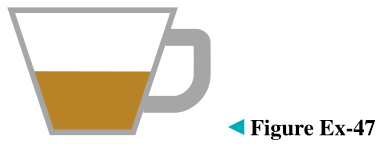
\includegraphics[width=0.4\textwidth]{../img/img_Lista3/47.png}
\end{figure}
Se vierte café a una velocidad uniforme de $20 cm^3/s$ en una taza cuyo interior tiene forma de cono truncado (consulte la figura adjunta). Si los radios superior e inferior de la taza son 4 cm y 2 cm y la altura de la taza es 6 cm, ¿con qué rapidez aumentará el nivel del café cuando el café esté a la mitad? [\textit{Sugerencia}: extienda la copa hacia abajo para formar un cono.]\\

Si extendemos la copa hacia abajo, con tal de formar un cono, donde $V_0$ sea el volumen de la porción agregada.

\begin{figure}[H]
\centering
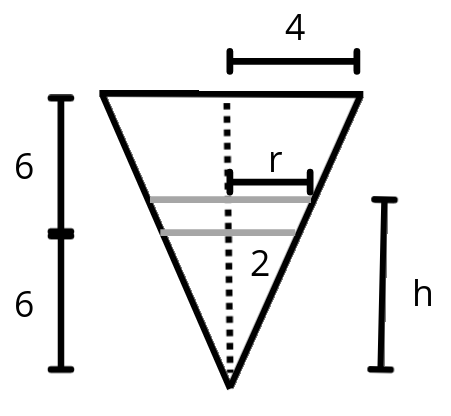
\includegraphics[width=0.35\textwidth]{../img/img_Lista3/cono.png}
\end{figure}

Primero calculamos el valor del radio
\[
\frac{r}{h}=\frac{4}{12}=\frac{1}{3}\qquad \therefore r=\frac{1}{3}h
\]

Así, tenemos entonces que el volumen es de

\[
V=\frac{1}{3}\pi r^2h-V_0 \underset{r=\frac{h}{3}}{\Longrightarrow} V=\frac{1}{27}\pi h^3-V_0
\]

Diferenciamos ambos lados de con respecto a $t$
\begin{align*}
  \frac{dV}{dt}
  &=\frac{1}{9}\pi h^2 \frac{dh}{dt}\\
\end{align*}

Entonces

\begin{align*}
  \frac{dh}{dt}
  &= \frac{9}{\pi h^2}\frac{dV}{dt}\\
\end{align*}

Sustituimos $\frac{dV}{dt}=20$ y evaluamos cuando $h=9$

\begin{align*}
  \frac{dh}{dt}\vline_{h=9}
  &= \frac{9}{\pi \cdot 9^2}\cdot 20\\
  &= \frac{20}{9\pi}
\end{align*}

$\therefore $ La rapidez con la que aumenta  el nivel del café cuando el café esté a la mitad es de
\[
\frac{20}{9\pi}\frac{cm}{s}
\]

%% 3.6 -----------------------------------------------------------------------------------------------------------------------------------------------------------------------------------------------------------------------------
\section{Sección 3.6 \\ La Regla De L'Hôpital; Formas Indeterminadas} 
% 58 -------------------------------------------------------------------------------------------------------------
\subsection{Ejercicio 58} Flores Morán Julieta Melina \\

Hay un mito que circula entre los estudiantes principiantes de cálculo que afirma que todas las formas indeterminadas de tipos $0^0,\infty^0$ y $1^{\infty}$ tienen valor 1 porque ''cualquier cosa elevada a cero es 1'' y ''1 elevado a cualquier potencia es 1''. La falacia es que $0^0,\infty^0$ y $1^{\infty}$ no son potencias de números, sino descripciones de límites. Los siguientes ejemplos, sugeridos por el Prof. Jack Staib de la Universidad de Drexel, muestran que estas formas indeterminadas pueden tener cualquier valor real positivo.
valor:
\begin{enumerate}[label=(\alph*)]
\item $\lim_{x \to 0^+} [x^{(\ln a)/(1+\ln x)}]=a \qquad$ (forma $0^0$)
\item $\lim_{x \to +\infty} [x^{(\ln a)/(1+\ln x)}]=a \qquad$ (forma $\infty^0$)
\item $\lim_{x \to 0} [(x+1)^{(\ln a)/x}]=a \qquad$ (forma $1^{\infty}$)
\end{enumerate}
Verifique estos resultados.


\begin{enumerate}[label=(\alph*)]
\item $\lim_{x \to 0^+} [x^{(\ln a)/(1+\ln x)}] \qquad$\\
Primero verifiquemos los límites de los factores.
\[
\lim_{x \to 0^+} x= 0
\]
\[
 \lim_{x \to 0^+} \frac{\ln a}{1+\ln x} =  \frac{\ln a}{1+  \lim_{x \to 0^+} \ln x}  =  \lim_{t \to \infty}  \frac{\ln a}{t} = 0
 \]
 Así que tenemos un tipo de indeterminación $0^{0}$ para la que podemos usar la regla de L'Hôpital.

 Ahora, por propiedades de los logaritmos.
 \[
 y =  x^{(\ln a)/(1+\ln x)}
 \]
  \[
 lny =  ln \left[x^{(\ln a)/(1+\ln x)}\right]
 \]
 Entonces
\[
   lny =  \frac{\ln a}{1+\ln x}   lnx
   \]
   \[
     \lim_{x \to 0^+} lny =  \frac{\ln a \cdot lnx}{1+\ln x}   
   \]
Y con esta información ya podemos sacar el límite de lny aplicando la regla de  L'Hôpital.
\begin{equation*}
  \begin{split}
    \lim_{x \to 0^+}lny
    &=  \lim_{x \to 0^+}  \frac{\ln a \cdot lnx}{1+\ln x}   \qquad\\
    &=  \lim_{x \to 0^+}  \frac{ \frac{d}{dx} [\ln a \cdot lnx]}{ \frac{d}{dx} [ 1+\ln x ]}   \qquad\\
    &=  \lim_{x \to 0^+}  \frac{ lna \cdot \frac{1}{x}}{  \frac{1}{x}}   \qquad\\
    &=  \lim_{x \to 0^+}  \frac{ lna}{1}   \qquad\\
  \therefore
   \lim_{x \to 0^+}lny
     &= lna \\
  \end{split}
\end{equation*}

Hemos demostrado que $lny   \rightarrow lna $ mientras $x \rightarrow 0^{+}$.La continuidad de la función exponencial implica que $e^{lny}  \rightarrow e^{lna} $ mientras   $x \rightarrow 0^{+}$. Lo que implica que $y \rightarrow a $.
\[
\therefore
\lim_{x \to 0^+} [x^{(\ln a)/(1+\ln x)}]=a \qquad 
\]

\item $\lim_{x \to +\infty} [x^{(\ln a)/(1+\ln x)}] \qquad$\\

Primero verifiquemos los límites de los factores.
\[
\lim_{x \to +\infty}  x= + \infty
\]
\[
\lim_{x \to +\infty}  \frac{\ln a}{1+\ln x} =  \frac{\ln a}{1+  \lim_{x \to +\infty} \ln x}  =  \lim_{t \to \infty}  \frac{\ln a}{t} = 0
 \]
 Así que tenemos un tipo de indeterminación $\infty ^{0}$ para la que podemos usar la regla de L'Hôpital.

 Ahora, por propiedades de los logaritmos.
 \[
 y =  x^{(\ln a)/(1+\ln x)}
 \]
  \[
 lny =  ln \left[x^{(\ln a)/(1+\ln x)}\right]
 \]
 Entonces
\[
   lny =  \frac{\ln a}{1+\ln x}   lnx
 \]
   \[
    \lim_{x \to +\infty}   lny =  \frac{\ln a \cdot lnx}{1+\ln x}   
   \]
Y con esta información ya podemos sacar el límite de lny aplicando la regla de  L'Hôpital.
\begin{equation*}
  \begin{split}
    \lim_{x \to +\infty} lny
    &= \lim_{x \to +\infty}   \frac{\ln a \cdot lnx}{1+\ln x}   \qquad\\
    &=  \lim_{x \to +\infty}  \frac{ \frac{d}{dx} [\ln a \cdot lnx]}{ \frac{d}{dx} [ 1+\ln x ]}   \qquad\\
    &=  \lim_{x \to +\infty}  \frac{ lna \cdot \frac{1}{x}}{  \frac{1}{x}}   \qquad\\
    &=  \lim_{x \to +\infty}   \frac{ lna}{1}   \qquad\\
  \therefore
   \lim_{x \to +\infty}  lny
     &= lna \\
  \end{split}
\end{equation*}

Hemos demostrado que $lny   \rightarrow lna $ mientras $x \rightarrow +\infty $.La continuidad de la función exponencial implica que $e^{lny}  \rightarrow e^{lna} $ mientras   $x \rightarrow +\infty$. Lo que implica que $y \rightarrow a $.
\[
\therefore
\lim_{x \to +\infty}   [x^{(\ln a)/(1+\ln x)}]=a \qquad 
\]
\item $\lim_{x \to 0} [(x+1)^{(\ln a)/x}] \qquad$ \\
Primero verifiquemos los límites de los factores.
\[
\lim_{x \to 0} x+1= 1
\]
\[
 \lim_{x \to 0} \frac{\ln a}{x} = \infty
 \]
 Así que tenemos un tipo de indeterminación $1^{\infty}$ para la que podemos usar la regla de L'Hôpital.

 Ahora, por propiedades de los logaritmos.
 \[
 y =  (x+1)^{(\ln a)/x}
 \]
  \[
 \ln y =  \ln \left[(x+1)^{(\ln a)/x}}\right]
 \]
 Entonces
\[
   \ln y =  \frac{\ln a}{x}  \ln (x+1)
   \]
   \[
     \lim_{x \to 0} \ln y =  \frac{\ln a \cdot  \ln (x+1)  }{x} 
   \]
Y con esta información ya podemos sacar el límite de $\ln y$ aplicando la regla de  L'Hôpital.
\begin{equation*}
  \begin{split}
    \lim_{x \to 0} \ln y
    &=  \lim_{x \to 0}  \frac{\ln a \cdot  \ln (x+1)} {x}   \qquad \\
    &=  \lim_{x \to 0}  \frac{ \frac{d}{dx} [\ln a \cdot  \ln (x+1)] } { \frac{d}{dx} [x] }   \qquad \\
    &=  \lim_{x \to 0}  \frac{ \ln a \cdot  \frac {1}{x+1} \cdot 1} { 1 }   \qquad \\
    &=  \lim_{x \to 0}  \frac{\ln a}{x+1} \qquad \\
    &=    \frac{\ln a}{0+1} \qquad \\
    &=    \frac{\ln a}{1} \qquad \\
  \therefore
   \lim_{x \to 0} \ln y
     &= lna \\
  \end{split}
\end{equation*}

Hemos demostrado que $lny   \rightarrow lna $ mientras $x \rightarrow 0$.La continuidad de la función exponencial implica que $e^{lny}  \rightarrow e^{lna} $ mientras   $x \rightarrow 0$. Lo que implica que $y \rightarrow a $.
\[
\therefore
\lim_{x \to 0} [(x+1)^{(\ln a)/x}]=a \qquad
\]

\end{enumerate}

% 63 -------------------------------------------------------------------------------------------------------------
\subsection{Ejercicio 63} Zarco Romero José Antonio \\

El diagrama esquemático adjunto representa un circuito eléctrico que consta de una fuerza electromotriz que produce un voltaje $V$, una resistencia con resistencia $R$ y un inductor con inductancia $L$. En la teoría de circuitos eléctricos se muestra que si el voltaje se aplica por primera vez en el momento $t = 0$, entonces la corriente $I$ que fluye a través del circuito en el tiempo $t$ está dada por
\[
I=\frac{V}{R}\left(1-e^{-Rt/L}\right)
\]

¿Cuál es el efecto sobre la corriente en un tiempo fijo $t$ si la resistencia se acerca a $0$ (es decir, $R\rightarrow 0^+$)?

\begin{figure}[H]
\centering
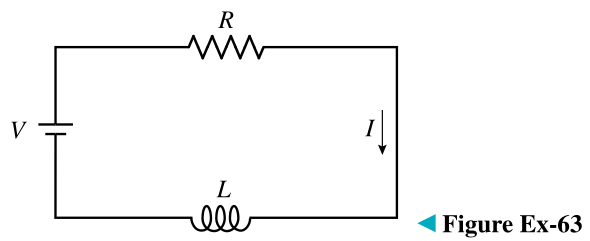
\includegraphics[width=0.7\textwidth]{../img/img_Lista3/circuit63.png}
\end{figure}

Para conocer el efecto sobre la corriente tenemos que calcular el límite de la ecuación cuando $R\rightarrow 0^+$, es decir
\begin{align*}
  \lim_{R \to 0^+} I
  &= \lim_{R \to 0^+} \frac{V}{R}\left(1-e^{-Rt/L}\right) \\
  &= \lim_{R \to 0^+} \frac{V \left(1-e^{-Rt/L}\right)}{R} \\
  &= \lim_{R \to 0^+} \frac{V-Ve^{-Rt/L}}{R} \\
\end{align*}

Dado que, el numerador y el denominador tienen un límite de 0, por lo que el límite es una forma indeterminada de tipo 0/0. Aplicando la regla de L'Hôpital se obtiene
\begin{align*}
  \lim_{R \to 0^+} I
  &= \lim_{R \to 0^+} \frac{\frac{d}{dt}[V-Ve^{-Rt/L}]}{\frac{d}{dt}[R]} \\
  &= \lim_{R \to 0^+} \frac{-Ve^{-Rt/L}\cdot \frac{d}{dt}[-Rt/L]}{1} \\
  &= \lim_{R \to 0^+} -Ve^{-Rt/L}\cdot -t/L \\
  &= \lim_{R \to 0^+} \frac{Vt}{L}e^{-Rt/L} \\ \\
  \therefore
  \lim_{R \to 0^+} I
  &= \frac{Vt}{L}
\end{align*}


% 65 -------------------------------------------------------------------------------------------------------------
\subsection{Ejercicio 65} Zarco Romero José Antonio \\

\begin{enumerate}[label=\alph*)]
\item Utilice un CAS para demostrar que si $k$ es una constante positiva, entonces
  \[
  \lim_{x \to +\infty} x(k^{1/x}-1)=\ln{k}
  \]
  
\begin{figure}[H]
\centering
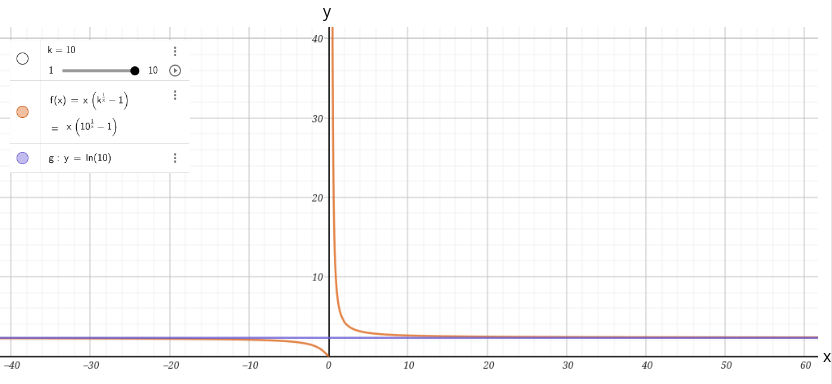
\includegraphics[width=1\textwidth]{../img/img_Lista3/cas65.png}
\end{figure}
  
\item Confirme este resultado utilizando la regla de L'Hôpital. [\textit{Sugerencia}: Exprese el límite en términos de $t = 1/x$.]

  El problema planteado es una forma indeterminada de tipo $\infty \cdot 0$. Lo convertiremos a una forma indeterminada de tipo 0/0:
  \begin{align*}
    \lim_{x \to +\infty} x(k^{1/x}-1)
    &= \lim_{x \to +\infty} \frac{k^{1/x}-1}{\frac{1}{x}} \\
    \text{Sea } t=\frac{1}{x}
    & \text{, entonces } t\rightarrow 0^+ \leftrightarrow x\rightarrow +\infty \\
    \lim_{t \to 0^+}
    &= \frac{k^t-1}{t} \\
    &= \frac{\frac{d}{dt}[k^t-1]}{\frac{d}{dt}[t]} \\
    &= \frac{k^t\ln{k}}{1} \\
    &= k^t\ln{k} \\
    \therefore
    \lim_{x \to +\infty} x(k^{1/x}-1)
    &= \ln{k} \\
  \end{align*}
  
\item Si $n$ es un entero positivo, entonces se deduce del inciso (a) con $x = n$ que la aproximación
  \[
  n(\sqrt[n]{k}-1)\approx \ln{k}
\]
debería ser bueno cuando $n$ es grande. Utilice este resultado y la tecla de raíz cuadrada en una calculadora para aproximar los valores de $\ln{0.3}$ y $\ln{2}$ con $n = 1024$, luego compare los valores obtenidos con los valores de los logaritmos generados directamente desde la calculadora. [\textit{Sugerencia}: Las raíces enésimas para las cuales $n$ es una potencia de 2 se pueden obtener como raíces cuadradas sucesivas.]

\begin{enumerate}
\item Calculadora: $\ln{0.3} = -1.20397\ldots$
  \begin{align*}
    1024(\sqrt[1024]{0.3}-1)
    &= 1024 \left[
      ((((((((((0.3)^{\frac{1}{2}})^{\frac{1}{2}})^{\frac{1}{2}})^{\frac{1}{2}})^{\frac{1}{2}})^{\frac{1}{2}})^{\frac{1}{2}})^{\frac{1}{2}})^{\frac{1}{2}})^{\frac{1}{2}}
      -1\right]\\
    &= 1024 \left[
      (((((((((0.54772\ldots)^{\frac{1}{2}})^{\frac{1}{2}})^{\frac{1}{2}})^{\frac{1}{2}})^{\frac{1}{2}})^{\frac{1}{2}})^{\frac{1}{2}})^{\frac{1}{2}})^{\frac{1}{2}}
      -1\right]\\
    &= 1024 \left[
      ((((((((0.74008\ldots)^{\frac{1}{2}})^{\frac{1}{2}})^{\frac{1}{2}})^{\frac{1}{2}})^{\frac{1}{2}})^{\frac{1}{2}})^{\frac{1}{2}})^{\frac{1}{2}}
      -1\right]\\
    &= 1024 \left[
      (((((((0.86028\ldots)^{\frac{1}{2}})^{\frac{1}{2}})^{\frac{1}{2}})^{\frac{1}{2}})^{\frac{1}{2}})^{\frac{1}{2}})^{\frac{1}{2}}
      -1\right]\\
    &= 1024 \left[
      ((((((0.92751\ldots)^{\frac{1}{2}})^{\frac{1}{2}})^{\frac{1}{2}})^{\frac{1}{2}})^{\frac{1}{2}})^{\frac{1}{2}}
      -1\right]\\
    &= 1024 \left[
      (((((0.96307\ldots)^{\frac{1}{2}})^{\frac{1}{2}})^{\frac{1}{2}})^{\frac{1}{2}})^{\frac{1}{2}}
      -1\right]\\
    &= 1024 \left[
      ((((0.98136\ldots)^{\frac{1}{2}})^{\frac{1}{2}})^{\frac{1}{2}})^{\frac{1}{2}}
      -1\right]\\
    &= 1024 \left[
      (((0.99063\ldots)^{\frac{1}{2}})^{\frac{1}{2}})^{\frac{1}{2}}
      -1\right]\\
    &= 1024 \left[
      ((0.99530\ldots)^{\frac{1}{2}})^{\frac{1}{2}}
      -1\right]\\
    &= 1024 \left[
      (0.99765\ldots)^{\frac{1}{2}}
      -1\right]\\
    &= 1024 \left[
      0.99882\ldots
      -1\right]\\
    &= 1024 [-0.00117\ldots] \\
    &= -1.20326\ldots \\ \\
    -1.20326\ldots \approx -1.20397\ldots\\ \\
    \therefore
    1024(\sqrt[1024]{0.3}-1)\approx \ln{0.3}
  \end{align*}
  
\item Calculadora: $\ln{2} = 0.693147\ldots$
  
  \begin{align*}
    1024(\sqrt[1024]{0.3}-1)
    &= 1024 \left[
      ((((((((((2)^{\frac{1}{2}})^{\frac{1}{2}})^{\frac{1}{2}})^{\frac{1}{2}})^{\frac{1}{2}})^{\frac{1}{2}})^{\frac{1}{2}})^{\frac{1}{2}})^{\frac{1}{2}})^{\frac{1}{2}}
      -1\right]\\
    &= 1024 \left[
      (((((((((1.41421\ldots)^{\frac{1}{2}})^{\frac{1}{2}})^{\frac{1}{2}})^{\frac{1}{2}})^{\frac{1}{2}})^{\frac{1}{2}})^{\frac{1}{2}})^{\frac{1}{2}})^{\frac{1}{2}}
      -1\right]\\
    &= 1024 \left[
      ((((((((1.18920\ldots)^{\frac{1}{2}})^{\frac{1}{2}})^{\frac{1}{2}})^{\frac{1}{2}})^{\frac{1}{2}})^{\frac{1}{2}})^{\frac{1}{2}})^{\frac{1}{2}}
      -1\right]\\
    &= 1024 \left[
      (((((((1.09050\ldots)^{\frac{1}{2}})^{\frac{1}{2}})^{\frac{1}{2}})^{\frac{1}{2}})^{\frac{1}{2}})^{\frac{1}{2}})^{\frac{1}{2}}
      -1\right]\\
    &= 1024 \left[
      ((((((1.0442\ldots)^{\frac{1}{2}})^{\frac{1}{2}})^{\frac{1}{2}})^{\frac{1}{2}})^{\frac{1}{2}})^{\frac{1}{2}}
      -1\right]\\
    &= 1024 \left[
      (((((1.02189\ldots)^{\frac{1}{2}})^{\frac{1}{2}})^{\frac{1}{2}})^{\frac{1}{2}})^{\frac{1}{2}}
      -1\right]\\
    &= 1024 \left[
      ((((1.01088\ldots)^{\frac{1}{2}})^{\frac{1}{2}})^{\frac{1}{2}})^{\frac{1}{2}}
      -1\right]\\
    &= 1024 \left[
      (((1.00542\ldots)^{\frac{1}{2}})^{\frac{1}{2}})^{\frac{1}{2}}
      -1\right]\\
    &= 1024 \left[
      ((1.00271\ldots)^{\frac{1}{2}})^{\frac{1}{2}}
      -1\right]\\
    &= 1024 \left[
      (1.00135\ldots)^{\frac{1}{2}}
      -1\right]\\
    &= 1024 \left[
      1.00067\ldots
      -1\right]\\
    &= 1024 [0.00067\ldots] \\
    &= 0.69338\ldots \\ \\
    0.69338\ldots \approx 0.693147\ldots\\ \\
    \therefore
    1024(\sqrt[1024]{2}-1)\approx \ln{2}
  \end{align*}
\end{enumerate}


\end{enumerate}

\end{document}
